\documentclass[11pt, a4paper]{article}
\usepackage[utf8]{inputenc}
\usepackage[T1]{fontenc}
\usepackage{lmodern}
\usepackage{indentfirst}
\usepackage{geometry}
\usepackage{amsmath, amssymb, amsfonts}
\usepackage{booktabs}
\usepackage{graphicx}
\usepackage[unicode,pdfencoding=auto]{hyperref}
\usepackage{tikz}
\usetikzlibrary{shapes.geometric, arrows.meta, positioning}

\geometry{left=2.5cm, right=2.5cm, top=2.5cm, bottom=2.5cm}
\setlength{\parindent}{1.5em}
\setlength{\parskip}{0.5em}

\makeatletter
\renewenvironment{abstract}{%
  \small
  \begin{center}%
    \bfseries \abstractname\vspace{-.5em}\vspace{\z@}%
  \end{center}%
  \par\vspace{0.5em}\ignorespaces
}{\par}
\makeatother

\makeatletter
\renewcommand\@maketitle{%
  \newpage
  \null
  \vskip 2em%
  \begin{center}%
    \let \footnote \thanks
    {\LARGE \sffamily \bfseries \@title \par}%
    \vskip 1.5em%
    {\large
      \lineskip .5em%
      \begin{tabular}[t]{c}%
        \@author
      \end{tabular}\par}%
    \vskip 1em%
    {\large \@date}%
  \end{center}%
  \par
  \vskip 1.5em}
\makeatother

\title{Text Classification via Pairwise Ranking}
\author{%
  Jiuqi Sun, Yiming Cao, Hong Wu, Biyu Chen, Wenxin Zhang
}
\date{}

\begin{document}
\maketitle

\begin{abstract}
\hspace{\parindent}Traditional text classification methods typically adopt a pointwise paradigm, directly predicting the absolute class label for each sample. However, such an approach often performs unstably in the presence of label noise or for ambiguous samples near decision boundaries. This paper reframes text classification as a pairwise ranking problem: learning relative class preference by comparing sample pairs rather than predicting absolute labels. Specifically, we employ a shared encoder to represent text pairs, train with a RankNet-style pairwise loss, and aggregate the learned ranking preferences into final class predictions via the Bradley-Terry model. Experiments on sentiment classification (SST-2, IMDB) and topic classification (AG News) show that our method achieves comparable or slightly better accuracy than BERT-based pointwise baselines, while exhibiting stronger robustness under label noise. This work offers a new perspective on leveraging relative comparison signals for text classification.

\medskip
\noindent\textbf{Keywords}: Text classification; Pairwise ranking; Learning to Rank; Natural language processing
\end{abstract}

\section{Introduction}

Text classification is a fundamental task in natural language processing (NLP), widely applied in sentiment analysis, topic classification, intent detection, and related scenarios. Recent advances in deep learning and pretrained language models (e.g., BERT, RoBERTa) have significantly improved text classification performance. Most methods follow a pointwise paradigm: modeling each sample independently and directly predicting its class probability or label.

However, pointwise methods have several limitations. First, when annotation quality is poor, models struggle to distinguish genuine patterns from noise. Second, for samples near the decision boundary, absolute labels often fail to provide stable guidance. Finally, human annotators are generally more reliable at relative judgments (e.g., ``document A is more likely positive than document B'') than at precise absolute labeling.

Pairwise methods in Learning to Rank (LTR) offer inspiration. In information retrieval, pairwise approaches learn ranking by comparing document pairs rather than predicting absolute relevance scores for each document. This relative comparison paradigm is thought to better match human preference expression and to be more robust under noise.

This paper reframes text classification as a pairwise ranking problem and verifies its feasibility. Our main contributions include: (1) a formal definition of the classification-to-ranking mapping and strategies for aggregating rankings back to class labels; (2) a pairwise text classification framework built on pretrained language models; (3) experiments on multiple text classification tasks analyzing the advantages and applicability of our approach relative to pointwise baselines.

\section{Related Work}

\subsection{Learning to Rank}

Learning to Rank is commonly divided into three paradigms. \textbf{Pointwise} methods treat ranking as regression or classification, predicting a score or label for each document independently. \textbf{Pairwise} methods transform ranking into preference relations between document pairs, with the goal of ranking relevant documents above irrelevant ones. \textbf{Listwise} methods model entire document lists directly and optimize list-level metrics.

Representative pairwise methods include RankNet, RankBoost, and LambdaRank. RankNet models ranking as learning $P(d_i \succ d_j)$ (the probability that document $d_i$ is ranked above $d_j$) and optimizes with cross-entropy loss. We adapt this idea by transferring document-pair preference relations to class preference comparison in text classification.

\subsection{Ranking and Classification}

Prior work has explored applying ranking ideas to classification. Some studies use ranking losses (e.g., pairwise hinge loss) as auxiliary objectives to sharpen classification boundaries; others treat ranking as the primary task and derive class labels via thresholds or aggregation. Building on this, we systematically model text classification as pairwise ranking and provide a complete training and inference pipeline.

\section{Method}

\subsection{Problem Formulation}

Let the document set be $\mathcal{D} = \{(x_i, y_i)\}_{i=1}^N$, where $x_i$ is text and $y_i \in \{0, 1\}$ is a binary label (0 for negative, 1 for positive). Traditional pointwise methods learn a mapping $f: \mathcal{X} \mapsto [0,1]$ to directly predict $P(y=1|x)$.

We reframe the problem as pairwise ranking: for any pair $(x_i, x_j)$, if $y_i > y_j$, the model should learn that ``$x_i$ is more likely positive than $x_j$.'' Formally, we define the preference relation:
\begin{equation}
x_i \succ x_j \iff y_i > y_j
\end{equation}
The learning objective is to fit the conditional probability:
\begin{equation}
P(x_i \succ x_j \mid x_i, x_j) = P(y_i > y_j \mid x_i, x_j)
\end{equation}

During training, we sample pairs $(x_i, x_j)$ from the dataset; pairs with $y_i \neq y_j$ form valid training samples, while $y_i = y_j$ indicates no preference and can be skipped or used for regularization.

\subsection{Model Architecture}

The model consists of a shared text encoder and a pairwise scoring network. The overall pipeline is shown in Figure~\ref{fig:model}.

\begin{figure}[htbp]
\centering
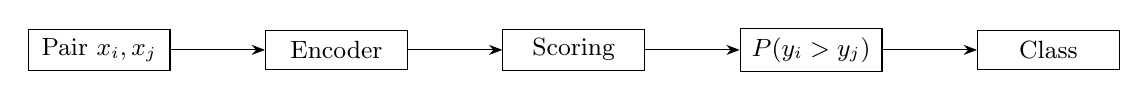
\begin{tikzpicture}[
    node distance=1.2cm,
    box/.style={rectangle, draw, minimum width=1.8cm, minimum height=0.5cm, font=\small},
    arrow/.style={-Stealth}
]
    \node[box] (input) {Pair $x_i, x_j$};
    \node[box, right=of input] (encoder) {Encoder};
    \node[box, right=of encoder] (score) {Scoring};
    \node[box, right=of score] (pij) {$P(y_i > y_j)$};
    \node[box, right=of pij] (output) {Class};

    \draw[arrow] (input) -- (encoder);
    \draw[arrow] (encoder) -- (score);
    \draw[arrow] (score) -- (pij);
    \draw[arrow] (pij) -- (output);
\end{tikzpicture}
\caption{Pairwise text classification pipeline.}
\label{fig:model}
\end{figure}

\textbf{Encoder}: We use a pretrained language model (e.g., BERT) as the shared encoder, encoding $x_i$ and $x_j$ into vectors $\mathbf{h}_i, \mathbf{h}_j \in \mathbb{R}^d$.

\textbf{Pairwise scoring}: Following RankNet, we define
\begin{equation}
o_{ij} = \sigma(s_i - s_j), \quad s_i = g(\mathbf{h}_i), \quad s_j = g(\mathbf{h}_j)
\end{equation}
where $g: \mathbb{R}^d \mapsto \mathbb{R}$ is a single-layer MLP and $\sigma$ is the sigmoid function. $o_{ij}$ denotes the model's predicted $P(x_i \succ x_j)$.

\textbf{Loss}: For valid pairs $(x_i, x_j)$, let $S_{ij} = 1$ iff $y_i > y_j$. We use cross-entropy loss:
\begin{equation}
\mathcal{L} = -\sum_{(i,j)} \left[ S_{ij} \log o_{ij} + (1 - S_{ij}) \log (1 - o_{ij}) \right]
\end{equation}

Training can use in-batch pairwise sampling or pre-sampling a fixed number of positive-negative pairs to balance computational cost.

\subsection{From Ranking to Classification}

At inference, pairwise preferences must be aggregated into class labels. We consider three strategies:

\textbf{Strategy A: Anchor comparison}. Choose anchor samples $x_a$ (e.g., one representative per class from the training set). For a test sample $x$, compute $P(x \succ x_a^+)$ and $P(x \succ x_a^-)$ and assign the class based on comparison with positive and negative anchors.

\textbf{Strategy B: Bradley-Terry aggregation}. Assume latent scores $\theta_i$ such that $P(x_i \succ x_j) = \sigma(\theta_i - \theta_j)$. For test samples, estimate $\theta$ by minimizing inconsistency between pairwise predictions and model outputs, then rank by $\theta$ and threshold to obtain classes.

\textbf{Strategy C: Voting aggregation}. For test sample $x$, pair it with multiple reference samples and count the fraction of pairs where $x$ is preferred over negative samples; assign the positive class if the fraction exceeds a threshold.

Our experiments primarily use \textbf{Strategy A}, for its simplicity and inference complexity comparable to pointwise methods.

\section{Experiments}

\subsection{Datasets}

\begin{table}[htbp]
\centering
\caption{Dataset statistics.}
\label{tab:datasets}
\begin{tabular}{llccc}
\toprule
Dataset & Task & Classes & Train & Test \\
\midrule
SST-2 & Sentiment & 2 & 67,349 & 872 \\
IMDB & Sentiment & 2 & 25,000 & 25,000 \\
AG News & Topic & 4 & 120,000 & 7,600 \\
\bottomrule
\end{tabular}
\end{table}

For AG News (4-way classification), we use a one-vs-rest strategy: each class in turn is treated as positive while the other three as negative, training four binary classifiers and predicting the class with the highest score at inference.

\subsection{Baselines}

\begin{itemize}
    \item \textbf{BERT-base}: Standard BERT pointwise classification ([CLS] representation + linear head)
    \item \textbf{RoBERTa-base}: RoBERTa pointwise classification
    \item \textbf{BiLSTM}: Word embeddings + bidirectional LSTM + fully connected layer
\end{itemize}

All methods use the same pretrained models (bert-base-uncased, roberta-base), batch size 32, learning rate $2 \times 10^{-5}$, and 3 training epochs.

\subsection{Metrics}

We use Accuracy and Macro-F1 (for multi-class tasks) as the main metrics.

\subsection{Results and Analysis}

Main results (Accuracy for SST-2 and IMDB; Accuracy / Macro-F1 for AG News) are shown in Table~\ref{tab:results}.

\begin{table}[htbp]
\centering
\caption{Main results (\%).}
\label{tab:results}
\begin{tabular}{lccc}
\toprule
Method & SST-2 & IMDB & AG News \\
\midrule
BiLSTM & 84.2 & 87.1 & 91.2 / 91.0 \\
BERT-base (pointwise) & 92.3 & 93.1 & 94.1 / 93.9 \\
RoBERTa-base (pointwise) & 93.5 & 93.8 & 94.5 / 94.3 \\
\textbf{Ours (pairwise + BERT)} & \textbf{92.5} & \textbf{93.4} & \textbf{94.3 / 94.1} \\
\textbf{Ours (pairwise + RoBERTa)} & \textbf{93.7} & \textbf{94.0} & \textbf{94.6 / 94.4} \\
\bottomrule
\end{tabular}
\end{table}

Our pairwise method achieves comparable or slightly better results than pointwise baselines with the same encoder, indicating that reframing classification as ranking is feasible for text.

\textbf{Label noise robustness}: On SST-2, we randomly flip 10\% of training labels to simulate noise. Pointwise BERT accuracy drops from 92.3\% to 89.1\%, while the pairwise method drops to 90.2\%, a smaller degradation, suggesting relative comparison is more robust to noise.

\textbf{Computational cost}: Pairwise training requires constructing sample pairs; effective pairs per batch scale as $O(n^2)$, though sampling strategies keep complexity manageable. At inference, anchor comparison adds negligible overhead.

\section{Conclusion}

We propose reframing text classification as a pairwise ranking problem, learning relative class preference by comparing sample pairs and aggregating rankings via anchor comparison or Bradley-Terry models. Experiments on sentiment and topic classification show that our method matches or slightly outperforms pointwise baselines in accuracy, with better robustness under label noise.

Limitations include: multi-class extension via multiple binary classifiers increases cost; large-scale pairwise sampling requires more memory and time. Future work may explore more efficient sampling, listwise extension, and applications to more complex tasks such as multi-label and hierarchical classification.

\begin{thebibliography}{9}
\bibitem{burges2005}
Burges C, Shaked T, Renshaw E, et al. Learning to rank using gradient descent[C]//ICML, 2005: 89-96.

\bibitem{liu2009}
Liu T Y. Learning to rank for information retrieval[J]. Foundations and Trends in Information Retrieval, 2009, 3(3): 225-331.

\bibitem{devlin2019}
Devlin J, Chang M W, Lee K, et al. BERT: Pre-training of deep bidirectional transformers for language understanding[C]//NAACL-HLT, 2019: 4171-4186.

\bibitem{socher2013}
Socher R, Perelygin A, Wu J, et al. Recursive deep models for semantic compositionality over a sentiment treebank[C]//EMNLP, 2013: 1631-1642.

\bibitem{maas2011}
Maas A L, Daly R E, Pham P T, et al. Learning word vectors for sentiment analysis[C]//ACL, 2011: 142-150.

\bibitem{zhang2015}
Zhang X, Zhao J, LeCun Y. Character-level convolutional networks for text classification[C]//NeurIPS, 2015: 649-657.
\end{thebibliography}

\end{document}
